\documentclass[a4paper,12pt]{article}
\usepackage[utf8]{inputenc}
\usepackage[T2A]{fontenc}
\usepackage[russian]{babel}
\usepackage{amsmath, amssymb, amsfonts}
\usepackage{graphicx}
\graphicspath{{../results/}{../}}
\usepackage{geometry}
\usepackage{hyperref}
\usepackage{float}
\usepackage{booktabs}
\usepackage{array}
\usepackage{subcaption}
\geometry{a4paper, top=2cm, bottom=2cm, left=2.5cm, right=1.5cm}

\begin{document}
	
	% Титульный лист
	\begin{titlepage}
		\begin{center}
			{\Large МОСКОВСКИЙ ГОСУДАРСТВЕННЫЙ УНИВЕРСИТЕТ \\ 
				имени М.В. ЛОМОНОСОВА}
			
			\vspace{0.5cm}
			{\Large МЕХАНИКО-МАТЕМАТИЧЕСКИЙ ФАКУЛЬТЕТ}
			
			\vspace{0.3cm}
			{\large Кафедра аэромеханики и газовой динамики}
			
			\vspace{3cm}
			
			{\Large \textbf{Задача по компьютерному практикуму}}
			
			\vspace{0.5cm}
			{\Large \textbf{Исследование дозвукового обтекания круглого цилиндра}}
			
			\vspace{0.5cm}
			{\large \textbf{на основе метода конформных отображений и полностью неявного метода}}
			
			\vspace{3cm}
			
			\begin{flushright}
				\large
				студент 5 курса \\
				Платонычев Иван Андреевич \\[1cm]
				Преподаватель по задаче: \\
				кандидат физико-математических наук \\
				Александр Николаевич Белоглазкин
			\end{flushright}
			
			\vspace{2cm}
			
			\begin{center}
				\large Москва \\
				\large 2026
			\end{center}
		\end{center}
	\end{titlepage}
	
	\newpage
	\tableofcontents
	\newpage
	
	\section{Постановка задачи}

\begin{figure}[h!]\centering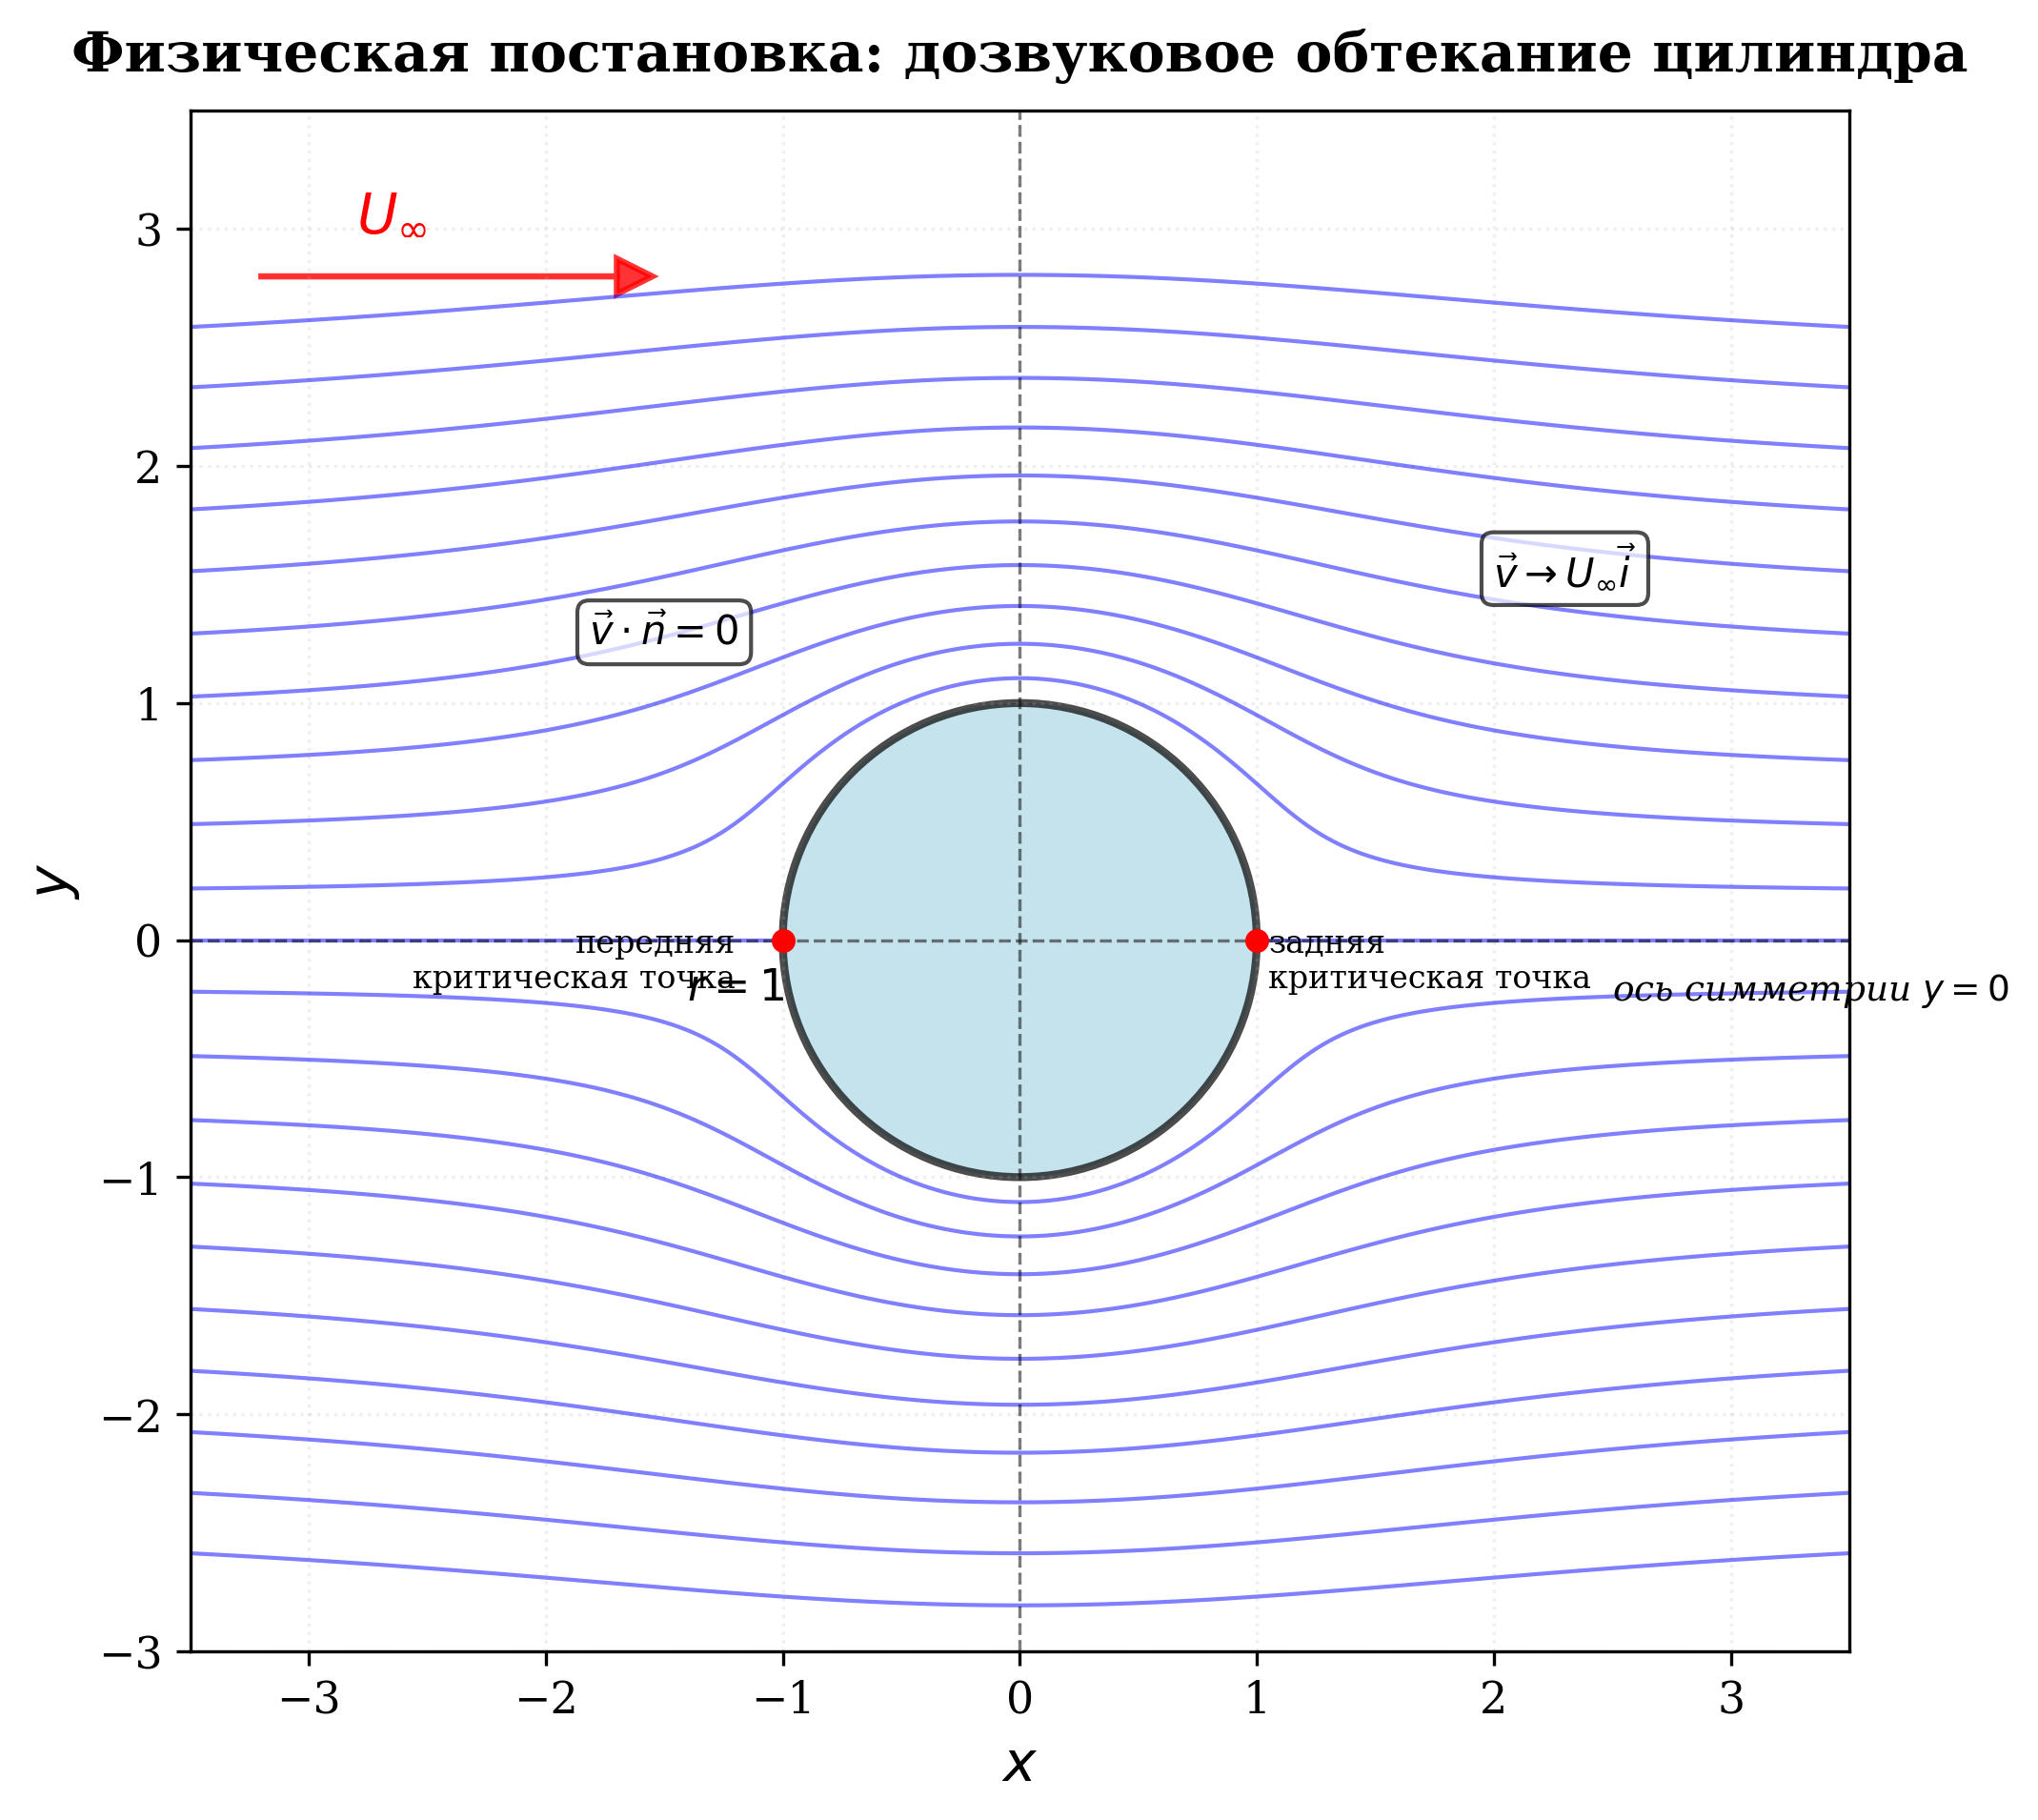
\includegraphics[width=0.4\textwidth]{1_physical_setup.png}\caption{Физическая постановка}\label{fig:setup}\end{figure}
	
	Рассматривается дозвуковое обтекание круглого цилиндра (рис. \ref{fig:setup}). В случае отсутствия завихренности стационарные двумерные уравнения Эйлера можно свести к нелинейному дифференциальному уравнению второго порядка в частных производных относительно потенциала скорости
	
	\[\vec{v} = \nabla \varphi.\]
	В декартовой системе координат имеем уравнение:
	
	\[
		\frac{\partial}{\partial x} \left( \rho \frac{\partial \varphi}{\partial x} \right) + \frac{\partial}{\partial y} \left( \rho \frac{\partial \varphi}{\partial y} \right) = 0,
	\]
	
	где плотность $\rho$ можно получить из условия изэнтропичности.
	
	На оси симметрии, на поверхности цилиндра задается условие непротекания
	
	

	\[\vec{v} \cdot \vec{n} = 0. \]	

	
	На больших расстояниях от цилиндра задается условие для невозмущенного потока
	
	
	\[ \vec{v}(r) \to U_{\infty} \vec{i} \quad \text{при} \quad r \to \infty.\]	
	
	
	В рамках данной постановки необходимо исследовать дозвуковое обтекание круглого цилиндра, используя конформное преобразование $\zeta = \ln z$, переводящее внешность единичной окружности на полуполосу $\xi \in [0, +\infty)$, $\eta \in [0, 2\pi]$.
	
	\textbf{Требуется}
	
	В рамках данной работы необходимо выполнить следующие задачи:
	
	\begin{enumerate}
		\item Вывести уравнения и соответствующие граничные условия в системе координат \((\xi, \eta)\).
		\item Составить разностную схему и решить ее с помощью ПНМ (Полностью Неявный Метод),
		сравнить данные по сходимости метода ПНМ с методом релаксации (неявную схема второго
		порядка по поперечной координате).
		\item В расчетной области для различных чисел Маха набегающего потока провести расчеты и сравнить распределение скорости и локального числа Маха.
		\item Исследовать зависимость результатов расчета от параметров сетки.
	\end{enumerate}
	
	\begin{thebibliography}{99}
		\bibitem{bai1961} Бай Ши-и, \textit{Введение в теорию течения сжимаемой жидкости}, ИЛ., М., 1961.
		\bibitem{buleev1959} Булеев Н.И. Численный метод решения двумерных уравнений диффузии // Атомная энергия, 1959, Том 6, № 3, С. 338–340.
		\bibitem{stone1968} Stone H.L. Iterative Solution of Implicit Approximations of Multidimensional Partial Differential Equations // SIAM Journal on Numerical Analysis, 1968, Vol. 5, No. 3, P. 530–558.
		\bibitem{pepper1977} D.W. Pepper, S.D. Harris, Fully Implicit Algorithms for Solving Partial Differential Equations // Journal of Fluids Engineering, 1977, 12, 781–783.
		\bibitem{beloglazkin1992} Белоглазкин А.Н., Шкадов В.Я. О влиянии проницаемости профиля на положение и интенсивность скачка при трансзвуковых скоростях // Вест. Моск. ун-та, сер. 1, математика, механика, 1992, № 5, С. 64–69.
	\end{thebibliography}
	\newpage
	
	\section{Уравнения Эйлера в размерном виде}
	
	Рассматривается стационарная задача, поэтому слагаемые, зависящие от времени, в уравнениях Эйлера опущены. Для описания течения сжимаемого газа используем систему уравнений Эйлера в размерном виде. Обозначим размерные величины со звездочкой $*$. 
	
	Уравнение неразрывности:
	\[
	\frac{\partial (\rho^* u^*)}{\partial x^*} + \frac{\partial (\rho^* v^*)}{\partial y^*} = 0.
	\]
	
	Уравнения движения (компоненты):
	\[
	\rho^* \left( u^* \frac{\partial u^*}{\partial x^*} + v^* \frac{\partial u^*}{\partial y^*} \right) = -\frac{\partial p^*}{\partial x^*},
	\]
	\[
	\rho^* \left( u^* \frac{\partial v^*}{\partial x^*} + v^* \frac{\partial v^*}{\partial y^*} \right) = -\frac{\partial p^*}{\partial y^*}.
	\]
	
	Уравнение энергии для изэнтропического течения:
	\[
	\frac{p^*}{\rho^{*\gamma}} = \text{const},
	\]
	где $\gamma$ — показатель адиабаты.
	
	Для стационарного безвихревого течения существует потенциал скорости $\varphi^*$, такой что:
	\[
	u^* = \frac{\partial \varphi^*}{\partial x^*}, \quad v^* = \frac{\partial \varphi^*}{\partial y^*}.
	\]
	
	Тогда уравнение неразрывности принимает вид:
	\[
	\frac{\partial}{\partial x^*} \left( \rho^* \frac{\partial \varphi^*}{\partial x^*} \right) + \frac{\partial}{\partial y^*} \left( \rho^* \frac{\partial \varphi^*}{\partial y^*} \right) = 0.
	\]
	
	Из условия изэнтропичности и интеграла Бернулли для безвихревого течения:
	\[
	\frac{\gamma}{\gamma-1} \frac{p^*}{\rho^*} + \frac{1}{2} \left( \frac{\partial \varphi^*}{\partial x^*} \right)^2 + \frac{1}{2} \left( \frac{\partial \varphi^*}{\partial y^*} \right)^2 = \text{const}.
	\]
	
	\subsection{Граничные условия в размерной постановке}
	
	\subsubsection{Условие непротекания на поверхности цилиндра}
	На поверхности цилиндра радиуса $R$ (в размерной форме) задается условие непротекания:
	\[
	\vec{v}^* \cdot \vec{n} = 0 \quad \text{при} \quad r^* = R,
	\]
	где $\vec{n}$ — единичный вектор нормали к поверхности цилиндра.
	
	В полярных координатах $(r^*, \theta)$ это условие записывается как:
	\[
	\frac{\partial \varphi^*}{\partial r^*} = 0 \quad \text{при} \quad r^* = R.
	\]
	
	\subsubsection{Условие на бесконечности}
	На больших расстояниях от цилиндра поток невозмущенный:
	\[
	\vec{v}^*(r^*) \to U_\infty^* \vec{i} \quad \text{при} \quad r^* \to \infty,
	\]
	где $U_\infty^*$ — скорость набегающего потока. В терминах потенциала скорости:
	\[
	\varphi^* \to U_\infty^* x^* \quad \text{при} \quad r^* \to \infty.
	\]
	
	\subsubsection{Условия симметрии}
	На оси симметрии ($y^* = 0$, $x^* \le -R$ и $x^* \ge R$) потенциал скорости является симметричной функцией:
	\[
	\varphi^*(x^*, y^*) = \varphi^*(x^*, -y^*) \quad \text{при} \quad y^* = 0, \; |x^*| \ge R.
	\]
	
	\section{Безразмерная постановка задачи}
	
	Для приведения системы уравнений Эйлера к безразмерному виду используем $\pi$-теорему теории размерности. В качестве основных масштабов выберем:
	\begin{itemize}
		\item Масштаб длины: $L = R$ — радиус цилиндра,
		\item Масштаб скорости: $U_\infty$ — скорость набегающего потока,
		\item Масштаб плотности: $\rho_\infty$ — плотность невозмущенного потока,
		\item Масштаб давления: $\rho_\infty U_\infty^2$.
	\end{itemize}
	
	Введем следующие безразмерные переменные:
	\[
	x = \frac{x^*}{L}, \quad y = \frac{y^*}{L}, \quad \varphi = \frac{\varphi^*}{U_\infty L}, \quad \rho = \frac{\rho^*}{\rho_\infty}, \quad p = \frac{p^*}{\rho_\infty U_\infty^2}.
	\]
	
	Размер расчетной области задан величиной $R_\infty = 5$. Основным варьируемым параметром задачи является число Маха набегающего потока $M_\infty$.
	
	\subsection{Безразмерные уравнения Эйлера}
	
	\subsubsection{Уравнение неразрывности}
	\[
	\frac{\partial (\rho u)}{\partial x} + \frac{\partial (\rho v)}{\partial y} = 0.
	\]
	
	\subsubsection{Уравнения движения (компоненты)}
	\[
	\rho \left( u \frac{\partial u}{\partial x} + v \frac{\partial u}{\partial y} \right) = -\frac{\partial p}{\partial x},
	\]
	\[
	\rho \left( u \frac{\partial v}{\partial x} + v \frac{\partial v}{\partial y} \right) = -\frac{\partial p}{\partial y}.
	\]
	
	\subsubsection{Уравнение для потенциала скорости}
	При условии безвихревости течения $\nabla \times \vec{v} = 0$ существует потенциал скорости $\vec{v} = \nabla \varphi$. Уравнение неразрывности в безразмерной форме принимает вид:
	\[
	\frac{\partial}{\partial x} \left( \rho \frac{\partial \varphi}{\partial x} \right) + \frac{\partial}{\partial y} \left( \rho \frac{\partial \varphi}{\partial y} \right) = 0.
	\]
	
	\subsubsection{Уравнение изэнтропичности и связь плотности с потенциалом}
	
	Из интеграла Бернулли для безвихревого изэнтропического течения:
	\[
	\frac{\gamma}{\gamma-1} \frac{p}{\rho} + \frac{1}{2} (u^2 + v^2) = \frac{\gamma}{\gamma-1} \frac{p_\infty}{\rho_\infty} + \frac{1}{2} U_\infty^2.
	\]
	
	С учетом изэнтропического соотношения $p / \rho^\gamma = \text{const}$ и переходя к безразмерным переменным, получим:
	\[
	\rho = \left[ 1 + \frac{\gamma-1}{2} M_\infty^2 \left( 1 - (u^2 + v^2) \right) \right]^{\frac{1}{\gamma-1}},
	\]
	where $M_\infty = U_\infty / a_\infty$ — число Маха набегающего потока, $a_\infty = \sqrt{\gamma p_\infty / \rho_\infty}$ — скорость звука в невозмущенном потоке.
	
	В терминах потенциала скорости:
	\[
	u = \frac{\partial \varphi}{\partial x}, \quad v = \frac{\partial \varphi}{\partial y},
	\]
	\[
	q^2 = u^2 + v^2 = \left( \frac{\partial \varphi}{\partial x} \right)^2 + \left( \frac{\partial \varphi}{\partial y} \right)^2.
	\]
	
	Таким образом, плотность выражается через потенциал скорости:
	\begin{equation}
		\boxed{\rho = \left[ 1 + \frac{\gamma-1}{2} M_\infty^2 \left( 1 - \left( \frac{\partial \varphi}{\partial x} \right)^2 - \left( \frac{\partial \varphi}{\partial y} \right)^2 \right) \right]^{\frac{1}{\gamma-1}}}
		\label{eq:density}
	\end{equation}
	
	\subsection{Безразмерные граничные условия}
	
	\subsubsection{Условие непротекания на поверхности цилиндра}
	На поверхности цилиндра $r = 1$ (в безразмерных координатах) нормальная компонента скорости равна нулю:
	\[
	\vec{v} \cdot \vec{n} = 0 \quad \text{при} \quad r = 1.
	\]
	В полярных координатах:
	\[
	\frac{\partial \varphi}{\partial r} = 0 \quad \text{при} \quad r = 1.
	\]
	
	\subsubsection{Условие на бесконечности}
	На больших расстояниях от цилиндра поток невозмущенный:
	\[
	\varphi \to x = r \cos \theta \quad \text{при} \quad r \to \infty.
	\]
	
	\subsubsection{Условия симметрии}
	На оси симметрии ($y = 0$, $|x| \ge 1$) потенциал скорости симметричен:
	\[
	\varphi(x, y) = \varphi(x, -y) \quad \text{при} \quad y = 0, \; |x| \ge 1.
	\]
	
	
	%%%%%%%%%%%%%%%%%%%%%%%%%%%%%%%%%
	\section{Преобразование координат и вывод уравнений в системе $(\xi, \eta)$}
	
	\subsection{Конформное преобразование}

	Введем комплексную переменную $z = x + iy$. Конформное отображение (рис. \ref{fig:mapping}), переводящее внешность единичной окружности в полуполосу, имеет вид:
	\begin{equation}
		\zeta = \ln z = \xi + i\eta,
	\end{equation}
	где $\xi = \ln |z| = \ln r$, $\eta = \arg z = \theta$.
	
	При таком преобразовании:
	\begin{itemize}
		\item Внешность единичной окружности $|z| \ge 1$ отображается в полуполосу $\xi \in [0, +\infty)$, $\eta \in [0, 2\pi)$.
		\item Поверхность цилиндра $|z| = 1$ отображается в линию $\xi = 0$.
		\item Бесконечно удаленная точка $|z| \to \infty$ отображается в $\xi \to +\infty$.
	\end{itemize}
	
	\subsection{Уравнение для потенциала скорости в координатах $(\xi, \eta)$}
	В декартовых координатах уравнение для потенциала скорости имеет вид:
	\[
	\frac{\partial}{\partial x} \left( \rho \frac{\partial \varphi}{\partial x} \right) + \frac{\partial}{\partial y} \left( \rho \frac{\partial \varphi}{\partial y} \right) = 0.
	\]
	
	Для конформного отображения $w = f(z)$ оператор Лапласа преобразуется как:
	\[
	\frac{\partial^2}{\partial x^2} + \frac{\partial^2}{\partial y^2} = |f'(z)|^2 \left( \frac{\partial^2}{\partial \xi^2} + \frac{\partial^2}{\partial \eta^2} \right).
	\]
	
	В нашем случае $f(z) = \ln z$, следовательно:
	\[
	f'(z) = \frac{1}{z} = e^{-\zeta} = e^{-\xi} e^{-i\eta}, \quad |f'(z)| = e^{-\xi}.
	\]
	
	Метрический коэффициент (якобиан) преобразования:
	\[
	J = |f'(z)|^{-2} = e^{2\xi}.
	\]
	
	Уравнение неразрывности в криволинейных координатах имеет вид:
	\[
	\frac{\partial}{\partial \xi} \left( \rho \frac{\partial \varphi}{\partial \xi} \right) + \frac{\partial}{\partial \eta} \left( \rho \frac{\partial \varphi}{\partial \eta} \right) = 0,
	\]
	где использовано соотношение $\sqrt{g} = |f'(z)|^{-1} = e^{\xi}$ и тот факт, что для конформного отображения коэффициенты Ламэ равны. Более подробный вывод приведен в Приложении.
	
	Окончательное уравнение в координатах $(\xi, \eta)$:
	\begin{equation}
		\boxed{\frac{\partial}{\partial \xi} \left( \rho \frac{\partial \varphi}{\partial \xi} \right) + \frac{\partial}{\partial \eta} \left( \rho \frac{\partial \varphi}{\partial \eta} \right) = 0}
	\end{equation}
	
	\subsection{Выражение для плотности через потенциал скорости}
	Из интеграла Бернулли и условия изэнтропичности связь между плотностью и скоростью имеет вид:
	\[
	\rho = \left[ 1 + \frac{\gamma-1}{2} M_\infty^2 \left( 1 - q^2 \right) \right]^{\frac{1}{\gamma-1}},
	\]
	где $q^2 = u^2 + v^2$ — квадрат модуля скорости.
	
	В координатах $(\xi, \eta)$ компоненты физической скорости выражаются через потенциал:
	\[
	u = \frac{\partial \varphi}{\partial x} = e^{-\xi} \left( \cos\eta \frac{\partial \varphi}{\partial \xi} - \frac{\sin\eta}{e^{\xi}} \frac{\partial \varphi}{\partial \eta} \right), \quad
	v = \frac{\partial \varphi}{\partial y} = e^{-\xi} \left( \sin\eta \frac{\partial \varphi}{\partial \xi} + \frac{\cos\eta}{e^{\xi}} \frac{\partial \varphi}{\partial \eta} \right).
	\]
	Квадрат скорости:
	\[
	q^2 = u^2 + v^2 = e^{-2\xi} \left[ \left( \frac{\partial \varphi}{\partial \xi} \right)^2 + \left( \frac{\partial \varphi}{\partial \eta} \right)^2 \right].
	\]
	
	\subsection{Граничные условия в координатах $(\xi, \eta)$}
	
	\subsubsection{Условие на поверхности цилиндра ($\xi = 0$)}
	На поверхности цилиндра $\xi = 0$ (твердая стенка) потенциал скорости $\varphi$ должен удовлетворять условию непротекания. В численной реализации это соответствует поведению потенциала вблизи границы, при котором его значения в фиктивных узлах за стенкой определяются через значения на самой границе:
	\[
	\varphi_{-1,j} = \varphi_{0,j}.
	\]
	
	\subsubsection{Условие на бесконечности ($\xi \to \infty$)}
	При $\xi \to \infty$ потенциал скорости стремится к потенциалу невозмущенного потока:
	\[
	\varphi \to e^{\xi} \cos \eta \quad \text{при} \quad \xi \to \infty.
	\]
	
	\subsubsection{Условия симметрии}
	В силу симметрии задачи потенциал скорости $\varphi(\xi, \eta)$ является четной периодической функцией по $\eta$ с периодом $2\pi$:
	\[
	\varphi(\xi, \eta) = \varphi(\xi, -\eta), \quad \varphi(\xi, \eta) = \varphi(\xi, 2\pi - \eta).
	\]
	Это позволяет рассматривать половину области $\eta \in [0, \pi]$ с условиями симметрии на границах $\eta=0$ и $\eta=\pi$.
	
	%%%%%%%%%%%%%%%%%%%%%%%%%%%%%%%
	%%%%%%%%%%%%%%%%%%%%%%55	

	\begin{figure}[H]
	\centering
	
\includegraphics[width=0.6\textwidth]{stencil_scheme.png}
	\caption{Разностная схема и шаблоны в расчетной области $(\xi, \eta)$. Показаны модификации шаблонов на границах: для твердой стенки ($\xi=0$), оси симметрии ($\eta=0, \pi$) и узлов перед бесконечностью.}
	\label{fig:stencil}
\end{figure}

\section{Полностью неявный метод (ПНМ)}
	
	Полностью неявный метод (ПНМ) основан на одновременном решении системы нелинейных разностных уравнений с использованием линеаризации Ньютона.


	
	\subsection{Формулировка разностного уравнения}
	Для внутреннего узла $(i,j)$, где $i = 1,\dots,N_\xi-1$, $j = 1,\dots,N_\eta-1$, разностное уравнение запишем в виде $F_{i,j} = 0$:
	\begin{equation}
		\begin{aligned}
			F_{i,j} = &\frac{1}{\Delta \xi^2} \left[ \rho_{i+\frac{1}{2},j} (\varphi_{i+1,j} - \varphi_{i,j}) - \rho_{i-\frac{1}{2},j} (\varphi_{i,j} - \varphi_{i-1,j}) \right] + \\
			&+ \frac{1}{\Delta \eta^2} \left[ \rho_{i,j+\frac{1}{2}} (\varphi_{i,j+1} - \varphi_{i,j}) - \rho_{i,j-\frac{1}{2}} (\varphi_{i,j} - \varphi_{i,j-1}) \right] = 0,
		\end{aligned}
		\label{eq:F}
	\end{equation}
	На границах области $F_{i,j}$ определяется соответствующими граничными условиями.
	
	%\subsubsection{Линеаризация по методу Ньютона}
	Пусть $\boldsymbol{\varphi}^{(k)}$ — приближенное решение на $k$-й итерации. Ищем поправку $\delta \boldsymbol{\varphi} = \boldsymbol{\varphi}^{(k+1)} - \boldsymbol{\varphi}^{(k)}$ такую, что:
	\[
	F_{i,j}(\boldsymbol{\varphi}^{(k)} + \delta \boldsymbol{\varphi}) = 0.
	\]
	Разлагая в ряд Тейлора с сохранением только линейных членов:
	\[
	F_{i,j}^{(k)} + \sum_{m,n} \frac{\partial F_{i,j}^{(k)}}{\partial \varphi_{m,n}} \delta \varphi_{m,n} = 0, \text{ где } F_{i,j}^{(k)} = F_{i,j}(\boldsymbol{\varphi}^{(k)}).
	\label{eq:newton_linear}
	\]

	
	В силу пятиточечной структуры схемы, $F_{i,j}$ зависит только от пяти узлов: $\varphi_{i-1,j}$, $\varphi_{i,j}$, $\varphi_{i+1,j}$, $\varphi_{i,j-1}$, $\varphi_{i,j+1}$. Поэтому уравнение (\ref{eq:newton_linear}) принимает вид:
	\begin{equation}
		\begin{aligned}
			& \frac{\partial F_{i,j}^{(k)}}{\partial \varphi_{i-1,j}} \delta \varphi_{i-1,j} + \frac{\partial F_{i,j}^{(k)}}{\partial \varphi_{i,j}} \delta \varphi_{i,j} + \frac{\partial F_{i,j}^{(k)}}{\partial \varphi_{i+1,j}} \delta \varphi_{i+1,j} +\\
			&+ \frac{\partial F_{i,j}^{(k)}}{\partial \varphi_{i,j-1}} \delta \varphi_{i,j-1} + \frac{\partial F_{i,j}^{(k)}}{\partial \varphi_{i,j+1}} \delta \varphi_{i,j+1} = - F_{i,j}^{(k)},
		\end{aligned}
		\label{eq:newton_system}
	\end{equation}
	
	\subsection{Вычисление производных}
	Для вычисления частных производных необходимо учесть, что плотность $\rho$ зависит от потенциала через градиенты. Введем обозначения:
	\[
	\rho = \rho(q^2), \quad q^2 = e^{-2\xi_i} \left[ \left( \frac{\partial \varphi}{\partial \xi} \right) ^2 + \left( \frac{\partial \varphi}{\partial \eta} \right) ^2 \right].
	\]
	Производные $\frac{\partial \rho}{\partial \varphi}$ вычисляются как сложная функция:
	\[
	\frac{\partial \rho}{\partial \varphi} = \frac{d\rho}{dq^2} \cdot \frac{\partial q^2}{\partial \varphi}.
	\]
	Из формулы для плотности (\ref{eq:density}):
	\[
	\frac{d\rho}{dq^2} = -\frac{\gamma-1}{2} M_\infty^2 \cdot \frac{\rho^{2-\gamma}}{\gamma-1} = -\frac{1}{2} M_\infty^2 \rho^{2-\gamma}.
	\]
	
	
	\subsection{Формирование разностной схемы }
	
	Для применения метода Стоуна систему линейных уравнений (\ref{eq:newton_system}) запишем в общем пятиточечном виде:
	\begin{equation}
		B_{i,j} \delta \varphi_{i,j-1} + D_{i,j} \delta \varphi_{i-1,j} + E_{i,j} \delta \varphi_{i,j} + F_{i,j} \delta \varphi_{i+1,j} + H_{i,j} \delta \varphi_{i,j+1} = q_{i,j},
		\label{eq:sip_stencil}
	\end{equation}
	где $q_{i,j} = -F_{i,j}^{(k)}$ — невязка на текущей итерации. Коэффициенты матрицы (в случае замороженной плотности) определяются выражениями:
	
	\begin{itemize}
		\item $B_{i,j} = \rho_{i,j-1/2} / \Delta \eta^2$ ,
		\item $D_{i,j} = \rho_{i-1/2,j} / \Delta \xi^2$ ,
		\item $F_{i,j} = \rho_{i+1/2,j} / \Delta \xi^2$ ,
		\item $H_{i,j} = \rho_{i,j+1/2} / \Delta \eta^2$ ,
		\item $E_{i,j} = -(B_{i,j} + D_{i,j} + F_{i,j} + H_{i,j})$.
	\end{itemize}

	\paragraph{Учет граничных условий в матрице:}
	Для реализации граничных условий в узлах, лежащих на границах расчетной области, используются модифицированные разностные уравнения. 
	
	\begin{enumerate}
		\item \textbf{Левая граница ($i=0$, поверхность цилиндра):} 
		Используется условие симметрии $\varphi_{-1,j} = \varphi_{0,j}$. Разностное уравнение (\ref{eq:sip_stencil}) для узлов $i=0$ принимает вид:
		\[ E_{0,j} \delta\varphi_{0,j} + F_{0,j} \delta\varphi_{1,j} + B_{0,j} \delta\varphi_{0,j-1} + H_{0,j} \delta\varphi_{0,j+1} = q_{0,j}, \]
		где коэффициенты определяются как:
		\[ E_{0,j} = -\left( \frac{\rho_{1/2,j}}{\Delta \xi^2} + \frac{\rho_{0,j+1/2} + \rho_{0,j-1/2}}{\Delta \eta^2} \right), \quad F_{0,j} = \frac{\rho_{1/2,j}}{\Delta \xi^2}, \quad D_{0,j} = 0. \]
		
		\item \textbf{Нижняя граница ($j=0$, ось симметрии):} 
		Используется условие $\varphi_{i,-1} = \varphi_{i,0}$. Уравнение для узлов $j=0$ (при $i > 0$):
		\[ E_{i,0} \delta\varphi_{i,0} + D_{i,0} \delta\varphi_{i-1,0} + F_{i,0} \delta\varphi_{i+1,0} + H_{i,0} \delta\varphi_{i,1} = q_{i,0}, \]
		где модифицированные коэффициенты:
		\[ E_{i,0} = -\left( \frac{\rho_{i+1/2,0} + \rho_{i-1/2,0}}{\Delta \xi^2} + \frac{\rho_{i,1/2}}{\Delta \eta^2} \right), \quad H_{i,0} = \frac{\rho_{i,1/2}}{\Delta \eta^2}, \quad B_{i,0} = 0. \]
		
		\item \textbf{Правая граница ($i=N_\xi$, бесконечность):} 
		Поскольку на бесконечности задано фиксированное значение потенциала (условие Дирихле), поправка в этих узлах должна быть равна нулю: $\delta \varphi_{N_\xi,j} = 0$. Это достигается установкой следующих коэффициентов:
		\[ E_{N_\xi,j} = 1, \quad B = D = F = H = 0, \quad q_{N_\xi,j} = 0. \]
	\end{enumerate}



	В глобальном векторе неизвестных система уравнений принимает вид $A \delta \boldsymbol{\varphi} = \mathbf{q}$, где матрица $A$ имеет характерную пятидиагональную структуру:
	\[
	A = \begin{pmatrix}
		E & F & 0 & \dots & H & & 0 \\
		D & E & F & \ddots & 0 & \ddots & \\
		0 & D & E & \ddots & \ddots & \ddots & H \\
		\vdots & 0 & \ddots & \ddots & \ddots & 0 & \vdots \\
		B & \ddots & \ddots & \ddots & E & F & 0 \\
		& \ddots & 0 & \ddots & D & E & F \\
		0 & & B & \dots & 0 & D & E 
	\end{pmatrix}
	\]
	Здесь диагонали $D$ и $F$ расположены непосредственно рядом с главной диагональю $E$, а диагонали $B$ и $H$ удалены от нее на расстояние, равное количеству узлов в строке сетки ($N_\xi+1$). Пространство между ними заполнено нулями, что отражает разреженность системы.

	
	\subsubsection{Алгоритм сильно неявной процедуры (SIP) Стоуна}
	
	Метод Стоуна \cite{stone1968} (Strongly Implicit Procedure) использует модифицированное неполное $LU$-разложение матрицы системы: $[A+N] \delta \boldsymbol{\varphi} = \mathbf{q}$, где матрица $N$ выбирается таким образом, чтобы аппроксимируемая система $[A+N]$ была близка к исходной $A$ и легко факторизовалась.
	
	Разложение ищется в виде произведения нижнетреугольной $L$ и верхнетреугольной $U$ матриц. Структурно они представляют собой разреженные матрицы с тремя ненулевыми диагоналями каждая (одна центральная и две смещенные):
	\[
	L = \begin{pmatrix}
		d_{i,j} & 0 & \dots \\
		c_{i,j} & d_{i+1,j} & 0 \\
		b_{i,j} & \dots & \ddots
	\end{pmatrix}, \quad
	U = \begin{pmatrix}
		1 & e_{i,j} & f_{i,j} \\
		0 & 1 & e_{i+1,j} \\
		\dots & 0 & 1
	\end{pmatrix}
	\]
	В терминах пятиточечного шаблона это можно записать как $L = [b_{i,j}, c_{i,j}, d_{i,j}]$ и $U = [1, e_{i,j}, f_{i,j}]$.

	\paragraph{Вычисление коэффициентов разложения:}
	Для каждого узла $(i,j)$ последовательно вычисляются коэффициенты $b, c, d, e, f$. Чтобы формулы были более читаемыми, используем дробную запись:
	\begin{equation}
		\displaystyle
		\left\{
		\begin{aligned}
			b_{i,j} &= \frac{B_{i,j}}{1 + \alpha e_{i,j-1}} \\[10pt]
			c_{i,j} &= \frac{D_{i,j}}{1 + \alpha f_{i-1,j}} \\[10pt]
			d_{i,j} &= E_{i,j} + \alpha (b_{i,j} e_{i,j-1} + c_{i,j} f_{i-1,j}) - b_{i,j} f_{i,j-1} - c_{i,j} e_{i-1,j} \\[10pt]
			e_{i,j} &= \frac{F_{i,j} - \alpha b_{i,j} e_{i,j-1}}{d_{i,j}} \\[10pt]
			f_{i,j} &= \frac{H_{i,j} - \alpha c_{i,j} f_{i-1,j}}{d_{i,j}}
		\end{aligned}
		\right.
	\end{equation}
	где $\alpha \in [0, 1]$ — параметр частичного учета влияния диагональных связей (обычно $\alpha \approx 0.92 \dots 0.95$).
	
	\paragraph{Решение системы (прямой и обратный ход):}
	После вычисления коэффициентов решение $\delta \varphi_{i,j}$ находится в два этапа:
	\begin{enumerate}
		\item \textbf{Прямой ход ($L\mathbf{y} = \mathbf{q}$):}
		\[ y_{i,j} = \frac{(q_{i,j} - b_{i,j} y_{i,j-1} - c_{i,j} y_{i-1,j})}{d_{i,j}}  . \]
		\item \textbf{Обратный ход ($U \delta \boldsymbol{\varphi} = \mathbf{y}$):}
		\[ \delta \varphi_{i,j} = y_{i,j} - e_{i,j} \delta \varphi_{i+1,j} - f_{i,j} \delta \varphi_{i,j+1}. \]
	\end{enumerate}
	
	Итерационный процесс продолжается до обеспечения малости поправки $\|\delta \varphi\|_\infty < \epsilon$. 
	
	\subsection{Пошаговый алгоритм решения}
	
	Реализация численного решения методом ПНМ включает следующие основные этапы:
	
	\begin{enumerate}
		\item \textbf{Инициализация:}
		\begin{itemize}
			\item Задание расчетной сетки и выбор начального приближения потенциала $\varphi^{(0)}$ (как правило, используется аналитическое решение для обтекания цилиндра \textit{несжимаемой} жидкостью).
			\item Установка фиксированных граничных условий на бесконечности (условие Дирихле) для заданного числа Маха $M_\infty$.
		\end{itemize}
		
		\item \textbf{Итерационный цикл (нахождение поправки $\delta\varphi$):}
		\begin{enumerate}
			\item \textbf{Обновление плотности:} Расчет поля плотности $\rho$ на основе текущих градиентов потенциала с использованием интеграла Бернулли.
			\item \textbf{Сборка матрицы:} Расчет невязок $q_{i,j}$ и коэффициентов пятиточечного шаблона $B, D, E, F, H$ с учетом условий непротекания на стенке и симметрии на оси.
			\item \textbf{Решение СЛАУ:} Нахождение поправок $\delta\varphi_{i,j}$ методом SIP (Стоуна).
			\item \textbf{Обновление решения:} $\varphi^{(k+1)} = \varphi^{(k)} + \delta \varphi$.
		\end{enumerate}
		
		\item \textbf{Контроль и постпроцессинг:}
		\begin{itemize}
			\item Проверка сходимости по норме поправки $\|\delta \varphi\|_\infty < \epsilon$.
			\item После достижения сходимости — расчет распределения давления $p$ и локальных чисел Маха $M_{loc}$ по всему полю.
		\end{itemize}
	\end{enumerate}



	\section{Метод последовательной строчной релаксации (SLOR)}

	В данной работе в качестве альтернативного решателя используется метод последовательной строчной релаксации (Successive Line Over-Relaxation). Основная идея метода заключается в одновременном уточнении значений потенциала вдоль целой строки сетки ($\eta = \text{const}$). 

	\subsection{Алгоритм метода}
	
	На каждой итерации $n$ производится последовательный обход строк $j = 0, \dots, N_\eta$. Для текущей строки $j$ значения потенциала в соседних строках ($j-1$ и $j+1$) считаются известными (используются значения с текущей или предыдущей итерации). Это приводит к системе уравнений для новой итерации $\varphi_{i,j}^{(n+1)}$ вдоль строки:
	
	\begin{equation}
		A_i \varphi_{i-1,j}^{(n+1)} + B_i \varphi_{i,j}^{(n+1)} + C_i \varphi_{i+1,j}^{(n+1)} = D_i, \quad i = 0, \dots, N_\xi
		\label{eq:slor_tridiag}
	\end{equation}
	
	Коэффициенты системы (\ref{eq:slor_tridiag}) определяются из аппроксимации уравнения неразрывности:
	
	\begin{itemize}
		\item $A_i = \displaystyle \frac{\rho_{i-1/2,j}}{\Delta \xi^2}$ — влияние предыдущего узла по $\xi$.
		\item $C_i = \displaystyle \frac{\rho_{i+1/2,j}}{\Delta \xi^2}$ — влияние следующего узла по $\xi$.
		\item $B_i = \displaystyle -\left( \frac{\rho_{i+1/2,j} + \rho_{i-1/2,j}}{\Delta \xi^2} + \frac{\rho_{i,j+1/2} + \rho_{i,j-1/2}}{\Delta \eta^2} \right)$ — центральный коэффициент.
		\item $D_i = \displaystyle - \frac{\rho_{i,j+1/2} \varphi_{i,j+1} + \rho_{i,j-1/2} \varphi_{i,j-1}}{\Delta \eta^2}$ — правая часть, содержащая вклады от соседних строк.
	\end{itemize}

	\paragraph{Учет граничных условий в методе SLOR:}
	
	Для граничных узлов трехдиагональная система уравнений (\ref{eq:slor_tridiag}) модифицируется следующим образом:
	
	\begin{enumerate}
		\item \textbf{Левая граница ($i=0$, поверхность цилиндра):} 
		С использованием условия $\varphi_{-1,j} = \varphi_{0,j}$ уравнение для первого узла строки принимает вид:
		\[ B_0 \varphi_{0,j}^{(n+1)} + C_0 \varphi_{1,j}^{(n+1)} = D_0, \]
		где коэффициенты:
		\[ B_0 = -\left( \frac{\rho_{1/2,j}}{\Delta \xi^2} + \frac{\rho_{0,j+1/2} + \rho_{0,j-1/2}}{\Delta \eta^2} \right), \quad C_0 = \frac{\rho_{1/2,j}}{\Delta \xi^2}. \]
		
		\item \textbf{Правая граница ($i=N_\xi$, бесконечность):} 
		Значение потенциала фиксировано: $\varphi_{N_\xi,j} = \varphi_{N_\xi,j}^\infty$. Это значение входит в правую часть уравнения для узла $i=N_\xi-1$:
		\[ A_{N_\xi-1} \varphi_{N_\xi-2,j}^{(n+1)} + B_{N_\xi-1} \varphi_{N_\xi-1,j}^{(n+1)} = D_{N_\xi-1} - C_{N_\xi-1} \varphi_{N_\xi,j}^\infty. \]
		
		\item \textbf{Нижняя и верхняя границы ($j=0, N_\eta$):} 
		За счет условий симметрии по $\eta$ ($\varphi_{i,-1} = \varphi_{i,0}$) правая часть $D_i$ для граничных строк содержит только вклад от внутренней соседней строки:
		\begin{itemize}
			\item При $j=0$: $D_i = \displaystyle - \frac{\rho_{i,1/2} \varphi_{i,1}}{\Delta \eta^2}$,
			\item При $j=N_\eta$: $D_i = \displaystyle - \frac{\rho_{i,N_\eta-1/2} \varphi_{i,N_\eta-1}}{\Delta \eta^2}$.
		\end{itemize}
	\end{enumerate}


	\subsection{Релаксация и сходимость}
	
	После нахождения решения системы (\ref{eq:slor_tridiag}), обозначим его $\tilde{\varphi}_{i,j}$. Окончательное значение в узле вычисляется с использованием параметра сверхрелаксации $\omega$:
	\begin{equation}
		\varphi_{i,j}^{(n+1)} = (1 - \omega) \varphi_{i,j}^{(n)} + \omega \tilde{\varphi}_{i,j}
	\end{equation}
	Для дозвуковых течений оптимальное значение $\omega$ обычно лежит в диапазоне $1.5 \dots 1.8$, что значительно ускоряет сходимость по сравнению с методом Гаусса-Зейделя ($\omega = 1$).

	\subsection{Пошаговый алгоритм решения}
	
	Реализация метода SLOR включает последовательное уточнение решения вдоль строк сетки:
	
	\begin{enumerate}
		\item \textbf{Подготовка:} Инициализация потенциала $\varphi$ и расчет начального поля плотности $\rho$.
		\item \textbf{Итерационный цикл:}
		\begin{itemize}
			\item Для каждой строки $j \in [0, N_\eta]$ выполняется:
			\begin{enumerate}
				\item Формирование элементов трехдиагональной матрицы $A_i, B_i, C_i$ и правой части $D_i$ с учетом текущих значений в соседних строках и граничных условий.
				\item \textbf{Решение прогонкой (алгоритм Томаса):} получение промежуточного значения $\tilde{\varphi}$ вдоль всей строки.
				\item \textbf{Сверхрелаксация:} $\varphi^{(n+1)} = (1 - \omega) \varphi^{(n)} + \omega \tilde{\varphi}$.
			\end{enumerate}
			\item Пересчет поля плотности $\rho$ после завершения прохода по всем строкам.
		\end{itemize}
		\item \textbf{Критерий остановки:} Расчет нормы невязки или максимальной поправки по всему полю: $\|\delta \varphi\|_\infty < \epsilon$.
	\end{enumerate}

	%%%%%%%%%%%%%%%%%%%%%%%%%%%
	\newpage
%\end{document}	
	\section{Вычисление физических величин}
	
	После нахождения потенциала скорости $\varphi(\xi, \eta)$ в расчетной области производится расчет физических характеристик потока.
	
	Связь между расчетными $(\xi, \eta)$ и физическими $(x, y)$ координатами:
	\begin{equation}
		x = e^\xi \cos \eta, \quad y = e^\xi \sin \eta.
	\end{equation}
	
	Квадрат модуля безразмерной скорости в каждой точке вычисляется через производные потенциала:
	\begin{equation}
		q^2 = e^{-2\xi} \left[ \left( \frac{\partial \varphi}{\partial \xi} \right)^2 + \left( \frac{\partial \varphi}{\partial \eta} \right)^2 \right].
	\end{equation}
	
	Локальное число Маха $M_{loc}$ определяется как отношение скорости к локальной скорости звука:
	\begin{equation}
		M_{loc} = \frac{q}{a}, \quad a^2 = \frac{1}{M_\infty^2} + \frac{\gamma-1}{2} (1 - q^2).
	\end{equation}
	
	Коэффициент давления $C_p$ рассчитывается по формуле для изэнтропического потока:
	\begin{equation}
		C_p = \frac{2}{\gamma M_\infty^2} \left( \rho^\gamma - 1 \right), \quad \text{где } \rho = \left[ 1 + \frac{\gamma-1}{2} M_\infty^2 (1 - q^2) \right]^{\frac{1}{\gamma-1}}.
	\end{equation}
	При $M_\infty \to 0$ (случай несжимаемой жидкости) формула для коэффициента давления переходит в классический вид:
	\begin{equation}
		C_p = 1 - q^2.
	\end{equation}

	\section{Результаты численного моделирования}

	В данном разделе представлены результаты расчетов для чисел Маха набегающего потока $M_\infty = 0.0, 0.1, 0.2, 0.3, 0.4$. Для обеспечения высокой точности и минимизации влияния внешних границ расчеты проводились на мелкой сетке $180 \times 150$ при удалении внешней границы $R_\infty = 50$.

	\subsection{Параметры потока и сходимость}

	В таблице \ref{tab:summary} приведены значения локального числа Маха и коэффициента давления в верхней точке цилиндра ($\theta = 90^\circ$), полученные методом ПНМ (SIP, $\alpha = 0.92$). Итерационный процесс проводился до достижения точности по поправке порядка $10^{-6}$ (около 2000 итераций для данной сетки).

	\begin{table}[H]
		\centering
		\caption{Сводная таблица результатов: ПНМ ($180 \times 150, R_\infty = 50$)}
		\label{tab:summary}
		\begin{tabular}{cccc}
			\toprule
			$M_\infty$ & $M_{loc, max}$ & $C_{p, min}$ & Итераций \\
			\midrule
			0.0 & 0.0000 & -2.9027 & 2000 \\
			0.1 & 0.1992 & -2.9247 & 2000 \\
			0.2 & 0.4097 & -2.9974 & 2000 \\
			0.3 & 0.6495 & -3.1478 & 2000 \\
			0.4 & 0.9737 & -3.4995 & 2000 \\
			\bottomrule
		\end{tabular}
	\end{table}

	\subsection{Эффективность ускоренного ПНМ}

	Для повышения скорости сходимости был реализован модифицированный вариант ПНМ («быстрый» ПНМ), использующий 20 внутренних итераций линейного решателя на каждом шаге уточнения плотности. В таблице \ref{tab:fast_comp} приведено сравнение количества внешних итераций для этого метода и метода SLOR.

	\begin{table}[H]
		\centering
		\caption{Сравнение производительности: Быстрый ПНМ и SLOR (сетка $120 \times 90$, $\epsilon=10^{-6}$)}
		\label{tab:fast_comp}
		\begin{tabular}{lcccc}
			\toprule
			$M_\infty$ & Итер. Fast-PNM & Итер. SLOR & $M_{loc, max}$ & Ускорение (по итер.) \\
			\midrule
			0.1 & 92 & 1316 & 0.1928 & 14.3x \\
			0.2 & 94 & 1333 & 0.3951 & 14.2x \\
			0.3 & 98 & 1365 & 0.6220 & 13.9x \\
			0.4 & 105 & 1420 & 0.9122 & 13.5x \\
			\bottomrule
		\end{tabular}
	\end{table}

	\subsection{Графики распределения параметров}

	На рисунках ниже представлены распределения локального числа Маха и коэффициента давления вдоль поверхности цилиндра, полученные методом ПНМ.

	\begin{figure}[H]
		\centering
		
\includegraphics[width=0.8\textwidth]{convergence_fast_only.png}
		\caption{Сходимость ускоренного метода (Fast SIP) для различных чисел Маха}
		\label{fig:conv_fast}
	\end{figure}

	\begin{figure}[H]
		\centering
		\begin{subfigure}{0.48\textwidth}
			
\includegraphics[width=\textwidth]{pnm_mach_M0.1.png}
			\caption{$M_\infty = 0.1$}
		\end{subfigure}
		\hfill
		\begin{subfigure}{0.48\textwidth}
			
\includegraphics[width=\textwidth]{pnm_mach_M0.2.png}
			\caption{$M_\infty = 0.2$}
		\end{subfigure}
		\\
		\begin{subfigure}{0.48\textwidth}
			
\includegraphics[width=\textwidth]{pnm_mach_M0.3.png}
			\caption{$M_\infty = 0.3$}
		\end{subfigure}
		\hfill
		\begin{subfigure}{0.48\textwidth}
			
\includegraphics[width=\textwidth]{pnm_mach_M0.4.png}
			\caption{$M_\infty = 0.4$}
		\end{subfigure}
		\caption{Распределение локального числа Маха на поверхности цилиндра (ПНМ)}
		\label{fig:pnm_mach}
	\end{figure}

	\subsection{Сравнение распределений числа Маха}

	Для дополнительной верификации приведено сравнение профилей локального числа Маха для обоих методов.

	\begin{figure}[H]
		\centering
		\begin{subfigure}{0.48\textwidth}
			
\includegraphics[width=\textwidth]{comp_mach_M0.1.png}
			\caption{$M_\infty = 0.1$}
		\end{subfigure}
		\hfill
		\begin{subfigure}{0.48\textwidth}
			
\includegraphics[width=\textwidth]{comp_mach_M0.2.png}
			\caption{$M_\infty = 0.2$}
		\end{subfigure}
		\\
		\begin{subfigure}{0.48\textwidth}
			
\includegraphics[width=\textwidth]{comp_mach_M0.3.png}
			\caption{$M_\infty = 0.3$}
		\end{subfigure}
		\hfill
		\begin{subfigure}{0.48\textwidth}
			
\includegraphics[width=\textwidth]{comp_mach_M0.4.png}
			\caption{$M_\infty = 0.4$}
		\end{subfigure}
		\caption{Сравнение локального числа Маха: ПНМ vs SLOR}
		\label{fig:comparison_mach}
	\end{figure}

	\subsection{Сравнение ПНМ и SLOR}

	Для верификации результатов проведено наложение профилей, полученных методами ПНМ и SLOR. Как видно из графиков, результаты практически идентичны, что подтверждает корректность обеих реализаций.

	\begin{figure}[H]
		\centering
		\begin{subfigure}{0.48\textwidth}
			
\includegraphics[width=\textwidth]{comp_cp_M0.1.png}
			\caption{$M_\infty = 0.1$}
		\end{subfigure}
		\hfill
		\begin{subfigure}{0.48\textwidth}
			
\includegraphics[width=\textwidth]{comp_cp_M0.2.png}
			\caption{$M_\infty = 0.2$}
		\end{subfigure}
		\\
		\begin{subfigure}{0.48\textwidth}
			
\includegraphics[width=\textwidth]{comp_cp_M0.3.png}
			\caption{$M_\infty = 0.3$}
		\end{subfigure}
		\hfill
		\begin{subfigure}{0.48\textwidth}
			
\includegraphics[width=\textwidth]{comp_cp_M0.4.png}
			\caption{$M_\infty = 0.4$}
		\end{subfigure}
		\caption{Сравнение коэффициента давления $C_p$: ПНМ (синяя линия) vs SLOR (красная пунктирная)}
		\label{fig:comparison}
	\end{figure}

	\subsection{История сходимости}

	На рисунке \ref{fig:conv_all} приведено сравнение скорости сходимости методов для всех рассмотренных чисел Маха.

	\begin{figure}[H]
		\centering
		
\includegraphics[width=0.8\textwidth]{convergence_all_updated.png}
		\caption{История сходимости $\|\delta \varphi\|_\infty$ для ускоренного ПНМ и метода SLOR (с указанием итераций)}
		\label{fig:conv_all}
	\end{figure}

	\begin{table}[H]
		\centering
		\caption{Сводная таблица сходимости и точности для всех методов и режимов}
		\label{tab:large_convergence}
		\begin{tabular}{llccccc}
			\toprule
			$M_\infty$ & Метод & Параметр & Итер. & Невязка & $M_{loc, max}$ & $C_p$ (min) \\
			\midrule
			0.1 & Fast PNM & $\alpha=0.92$ & 92 & $2.2\cdot 10^{-6}$ & 0.1928 & -2.6771 \\
			    & SLOR     & $\omega=1.70$ & 1316 & $1.1\cdot 10^{-6}$ & 0.1928 & -2.6771 \\
			\midrule
			0.2 & Fast PNM & $\alpha=0.92$ & 94 & $2.6\cdot 10^{-6}$ & 0.3951 & -2.7365 \\
			    & SLOR     & $\omega=1.70$ & 1333 & $1.2\cdot 10^{-6}$ & 0.3951 & -2.7365 \\
			\midrule
			0.3 & Fast PNM & $\alpha=0.92$ & 98 & $3.7\cdot 10^{-6}$ & 0.6220 & -2.8562 \\
			    & Stand. PNM & $\alpha=0.92$ & 1412 & $1.0\cdot 10^{-6}$ & 0.6219 & -2.8560 \\
			    & Stand. PNM & $\alpha=0.00$ & 4944 & $1.0\cdot 10^{-6}$ & 0.6218 & -2.8544 \\
			    & SLOR     & $\omega=1.70$ & 1365 & $1.4\cdot 10^{-6}$ & 0.6220 & -2.8563 \\
			    & SLOR     & $\omega=1.00$ & 4429 & $1.0\cdot 10^{-6}$ & 0.6218 & -2.8549 \\
			\midrule
			0.4 & Fast PNM & $\alpha=0.92$ & 105 & $2.9\cdot 10^{-6}$ & 0.9122 & -3.1119 \\
			    & SLOR     & $\omega=1.70$ & 1420 & $1.1\cdot 10^{-6}$ & 0.9122 & -3.1119 \\
			\bottomrule
		\end{tabular}
	\end{table}

	\subsection{Влияние параметров методов на сходимость}

	Исследовано влияние параметров релаксации $\omega$ (для SLOR) и параметра $\alpha$ (для SIP) на скорость и факт сходимости для $M_\infty = 0.3$ на сетке $120 \times 90$.

	\begin{table}[H]
		\centering
		\caption{Сравнение параметров стандартных методов ($M_\infty = 0.3$, сетка $120 \times 90$, $\epsilon=10^{-7}$)}
		\label{tab:params}
		\begin{tabular}{lccccc}
			\toprule
			Метод & Параметр & Невязка & $M_{loc, max}$ & $C_p$ (min) & Итерации \\
			\midrule
			SIP & $\alpha = 0.92$ & $9.9\cdot 10^{-7}$ & 0.6219 & -2.8560 & 1412 \\
			SIP & $\alpha = 0.00$ & $9.9\cdot 10^{-7}$ & 0.6218 & -2.8544 & 4944 \\
			SLOR & $\omega = 1.70$ & $9.9\cdot 10^{-7}$ & 0.6220 & -2.8563 & 1365 \\
			SLOR & $\omega = 1.00$ & $9.9\cdot 10^{-7}$ & 0.6218 & -2.8549 & 4429 \\
			\bottomrule
		\end{tabular}
	\end{table}

	Влияние параметров на сходимость ускоренного ПНМ приведено в таблице \ref{tab:fast_params}.

	\begin{table}[H]
		\centering
		\caption{Влияние параметров на сходимость быстрого ПНМ ($M_\infty = 0.3$, $\epsilon=10^{-6}$)}
		\label{tab:fast_params}
		\begin{tabular}{lcc}
			\toprule
			Метод и параметр & Итерации (внешние) & Остаточная невязка \\
			\midrule
			FastSIP ($\alpha = 0.92$) & 98 & $3.7 \cdot 10^{-6}$ \\
			FastSIP ($\alpha = 0.00$) & 340 & $2.0 \cdot 10^{-6}$ \\
			SLOR ($\omega = 1.70$) & 1365 & $1.4 \cdot 10^{-6}$ \\
			SLOR ($\omega = 1.00$) & 4429 & $1.0 \cdot 10^{-6}$ \\
			\bottomrule
		\end{tabular}
	\end{table}

	На рисунке \ref{fig:conv_M03} показана детальная история сходимости для различных параметров при $M_\infty = 0.3$. Видно, что при $\alpha=0.92$ и $\omega=1.7$ наблюдается значительно более быстрая минимизация невязки.
	\begin{figure}[H]
		\centering
		
\includegraphics[width=0.8\textwidth]{convergence_M0.3_updated.png}
		\caption{История сходимости для различных параметров методов ($M_\infty = 0.3$, до 5000 итераций)}
		\label{fig:conv_M03}
	\end{figure}

	\subsection{Критическое значение числа Маха}

	При увеличении числа Маха набегающего потока $M_\infty$ локальное число Маха в верхней точке цилиндра ($\theta = 90^\circ$) также возрастает. Критическим числом Маха $M_{cr}$ называется такое значение $M_\infty$, при котором локальная скорость в какой-либо точке поверхности впервые достигает скорости звука ($M_{loc} = 1.0$). 

	Для поиска этого значения были проведены дополнительные расчеты в окрестности $M_\infty = 0.425$ на сетке $60 \times 45$. Результаты представлены в таблице \ref{tab:critical}.

	\begin{table}[H]
		\centering
		\caption{Результаты расчета в окрестности критического числа Маха}
		\label{tab:critical}
		\begin{tabular}{lccccc}
			\toprule
			$M_\infty$ & $M_{loc, max}$ & $C_p$ (min) & Итер. PNM & Итер. SLOR & Сходимость \\
			\midrule
			0.420 & 0.9709 & -3.1028 & 75 & 960 & Да \\
			\textbf{0.425} & \textbf{0.9906} & \textbf{-3.1262} & \textbf{75} & \textbf{962} & \textbf{Да} \\
			0.430 & 1.0111 & -3.1514 & 75 & 964 & Да* \\
			\bottomrule
		\end{tabular}
	\end{table}

	Как видно из результатов, при $M_\infty = 0.425$ локальное число Маха на вершине цилиндра достигает $\approx 0.99$, что практически соответствует критическому режиму. При $M_\infty = 0.430$ в потоке уже возникают локальные сверхзвуковые зоны ($M_{loc} > 1.0$). 

	\begin{figure}[H]
		\centering
		
\includegraphics[width=0.7\textwidth]{transonic_cylinder_mach_distribution.png}
		\caption{Визуализация распределения числа Маха при $M_\infty \approx M_{cr} = 0.425$. Белая линия (изолиния $M=1.0$) ограничивает зарождающуюся сверхзвуковую зону (supersonic pocket).}
		\label{fig:transonic}
	\end{figure}

	Важно отметить, что при $M_\infty > M_{cr}$ используемая в работе численная схема (как ПНМ, так и SLOR) теряет устойчивость или сходится к нефизичному решению. Это связано с тем, что уравнение для потенциала скорости (\ref{eq:F}) является эллиптическим только в дозвуковой области. При появлении сверхзвуковых зон ($M_{loc} > 1$) уравнение меняет тип на гиперболический.

	\subsection{Влияние удаления внешней границы на критическое число Маха}

	Для оценки влияния размеров расчетной области было проведено исследование зависимости критического числа Маха $M_{cr}$ от радиуса внешней границы $R_\infty$. Результаты приведены в таблице \ref{tab:r_study}.

	\begin{table}[H]
		\centering
		\caption{Зависимость критического числа Маха от радиуса внешней границы $R_\infty$}
		\label{tab:r_study}
		\begin{tabular}{ccc}
			\toprule
			$R_\infty$ & $M_{cr}$ & $M_{loc, max}$ \\
			\midrule
			1.5 & 0.660 & 1.0183 \\
			2.0 & 0.550 & 1.0514 \\
			2.5 & 0.500 & 1.0633 \\
			3.0 & 0.470 & 1.0526 \\
			3.5 & 0.450 & 1.0344 \\
			4.0 & 0.450 & 1.0858 \\
			4.5 & 0.450 & 1.1356 \\
			5.0 & 0.421 & 1.0006 \\
			5.5 & 0.418 & 1.0023 \\
			6.0 & 0.415 & 1.0002 \\
			6.5 & 0.413 & 0.9999 \\
			7.0 & 0.412 & 1.0023 \\
			7.5 & 0.411 & 1.0032 \\
			8.0 & 0.410 & 1.0030 \\
			8.5 & 0.409 & 1.0020 \\
			9.0 & 0.408 & 1.0003 \\
			9.5 & 0.408 & 1.0028 \\
			10.0 & 0.407 & 1.0002 \\
			\bottomrule
		\end{tabular}
	\end{table}

	Из таблицы видно, что при малых $R_\infty$ значение критического числа Маха завышено, что объясняется стеснением потока границами области. С ростом $R_\infty$ значение $M_{cr}$ стабилизируется в районе $0.407 \dots 0.410$.

	\appendix
	\section{Приложение: Вывод уравнения в координатах $(\xi, \eta)$}	
	Уравнение неразрывности в полярных координатах:
	\[
	\frac{1}{r} \frac{\partial}{\partial r} \left( \rho r \frac{\partial \varphi}{\partial r} \right) + \frac{1}{r^2} \frac{\partial}{\partial \theta} \left( \rho \frac{\partial \varphi}{\partial \theta} \right) = 0.
	\]
	Переходя к переменным $(\xi, \eta)$ с учетом $\frac{\partial}{\partial r} = e^{-\xi} \frac{\partial}{\partial \xi}$, $\frac{\partial}{\partial \theta} = \frac{\partial}{\partial \eta}$, $r = e^{\xi}$:
	\[
	\frac{\partial}{\partial \xi} \left( \rho \frac{\partial \varphi}{\partial \xi} \right) + \frac{\partial}{\partial \eta} \left( \rho \frac{\partial \varphi}{\partial \eta} \right) = 0.
	\]

\end{document}